\documentclass[10pt, aspectratio=169]{beamer}

% Pacotes de Idioma e Matemática
\usepackage[brazilian]{babel}
\usepackage[utf8]{inputenc}
\usepackage[T1]{fontenc}
\usepackage{amsmath,amssymb,amsthm}
\usepackage{graphicx}
\usepackage{booktabs}
\usepackage{tcolorbox}

% --- PALETA DE CORES INSTITUCIONAL (IFPE) ---
\definecolor{primary}{RGB}{14, 114, 52}     % Verde IFPE
\definecolor{secondary}{RGB}{10, 80, 36}    % Verde Escuro Destaque
\definecolor{darkgrey}{RGB}{50, 50, 50}     % Cinza Escuro
\definecolor{bglight}{RGB}{245, 247, 250}   % Cinza Claro

% --- CONFIGURAÇÕES DO TEMA BEAMER ---
\usetheme{Boadilla}
\usecolortheme{default}

\setbeamercolor{structure}{fg=primary}
\setbeamercolor{palette primary}{bg=primary, fg=white}
\setbeamercolor{palette secondary}{bg=secondary, fg=white}
\setbeamercolor{palette tertiary}{bg=primary!80, fg=white}
\setbeamercolor{titlelike}{bg=primary, fg=white}
\setbeamercolor{frametitle}{bg=primary, fg=white}
\setbeamercolor{block title}{bg=secondary, fg=white}
\setbeamercolor{block body}{bg=bglight, fg=black}

\setbeamertemplate{navigation symbols}{}

% Rodapé Personalizado
\setbeamertemplate{footline}{
  \leavevmode%
  \hbox{%
  \begin{beamercolorbox}[wd=.333333\paperwidth,ht=2.25ex,dp=1ex,center]{author in head/foot}%
    \usebeamerfont{author in head/foot}Prof. Cleibson José da Silva
  \end{beamercolorbox}%
  \begin{beamercolorbox}[wd=.333333\paperwidth,ht=2.25ex,dp=1ex,center]{title in head/foot}%
    \usebeamerfont{title in head/foot}Matemática -- IFPE
  \end{beamercolorbox}%
  \begin{beamercolorbox}[wd=.333333\paperwidth,ht=2.25ex,dp=1ex,right]{date in head/foot}%
    \usebeamerfont{date in head/foot}\insertframenumber{} / \inserttotalframenumber\hspace*{2ex} 
  \end{beamercolorbox}}%
  \vskip0pt%
}

% --- DADOS DA APRESENTAÇÃO ---
\title[Polinômios I]{Polinômios -- Parte I}
\subtitle{Definição, Grau, Identidade, Raiz e Operações Básicas}
\author[Prof. Cleibson]{Prof. Cleibson José da Silva}
\institute[IFPE]{Instituto Federal de Pernambuco -- Campus Caruaru\\
\vspace{0.2cm}
  \IfFileExists{Imagens/logocaruaru.png}{
\includegraphics[height=2cm]{Imagens/logocaruaru.png}}{\textbf{IFPE Campus Caruaru}}
}
\date{}

\begin{document}

% Slide de Título
\begin{frame}
  \titlepage
\end{frame}

% Definição de Polinômio
\begin{frame}{Definição de Polinômio}
  \begin{block}{Definição Formal}<1->
    Um \textbf{polinômio} é uma função na variável $x$ da forma:
    \[
      P(x) = a_n x^n + a_{n-1} x^{n-1} + \dots + a_1 x + a_0
    \]
    Em que:
    \begin{itemize}
      \item $a_n, a_{n-1}, \dots, a_1, a_0$ são os \textbf{coeficientes} reais ou complexos.
      \item Os expoentes são números naturais ($n \in \mathbb{N}$).
    \end{itemize}
  \end{block}

  \pause

  \begin{alertblock}{Polinômio Nulo}<2->
    Um polinômio é dito \textbf{nulo} se todos os seus coeficientes são iguais a zero:
    \[
      P(x) \equiv 0 \iff a_n = a_{n-1} = \dots = a_1 = a_0 = 0
    \]
  \end{alertblock}
\end{frame}

% Exemplos de Polinômios
\begin{frame}{Exemplos de Polinômios}
  \begin{exampleblock}{Exemplos da Apostila}
    \begin{enumerate}[<+->]
      \item $P(x) = 3x^4 - 7x^3 + 8x + 2$
      \item $P(x) = -4x^5 + 8x^4 - 9x^3 + 18x^2 + 7x - 1$
      \item $P(x) = 5$ \quad (Polinômio constante)
    \end{enumerate}
  \end{exampleblock}
\end{frame}

% Grau do Polinômio
\begin{frame}{Grau do Polinômio}
  \begin{block}{Definição do Grau}<1->
    Considere $P(x) = a_n x^n + a_{n-1} x^{n-1} + \dots + a_1 x + a_0$.
    
    Dizemos que o grau de $P(x)$ (indica-se por $\text{gr}(P)$ ou $\partial P$) é igual a $n$ se $a_n \neq 0$.
  \end{block}

  \pause

  \begin{exampleblock}{Exemplos da Apostila}<2->
    \begin{itemize}[<+->]
      \item O grau de $P(x) = 7x^4 - 3x^2 + 8$ é igual a $4$.
      \item O grau de $P(x) = 2x^2 + 8$ é igual a $2$.
      \item O grau de $P(x) = 13$ é igual a $0$.
    \end{itemize}
  \end{exampleblock}

  \pause

  \begin{alertblock}{Observação Importante}<5->
    \textbf{Não se define} o grau de um polinômio nulo.
  \end{alertblock}
\end{frame}

% Polinômios Idênticos: Conceito
\begin{frame}{Polinômios Idênticos}
  \begin{block}{Definição}<1->
    Os polinômios 
    \[ P(x) = a_n x^n + \dots + a_1 x + a_0 \quad \text{e} \quad Q(x) = b_n x^n + \dots + b_1 x + b_0 \]
    são \textbf{idênticos} ($P(x) \equiv Q(x)$) se, e somente se, os coeficientes dos termos correspondentes forem iguais.
  \end{block}

  \pause

  \begin{block}{Condição de Igualdade}<2->
    \[
      a_n = b_n, \quad a_{n-1} = b_{n-1}, \quad \dots, \quad a_1 = b_1 \quad \text{e} \quad a_0 = b_0
    \]
  \end{block}
\end{frame}

% Polinômios Idênticos: Exemplo
\begin{frame}{Exemplo: Polinômios Idênticos}
  \begin{exampleblock}{Exemplo da Apostila}
    Determinar os valores de $a$, $b$ e $c$ para os quais os polinômios
    \[
      P(x) = ax^2 + 3x + 9 \quad \text{e} \quad B(x) = (b+3)x^2 + (c-1)x + 3b
    \]
    são idênticos.
  \end{exampleblock}

\end{frame}

% Raiz ou Zero de um Polinômio
\begin{frame}{Raiz ou Zero de um Polinômio}
  \begin{block}{Definição Formal}<1->
    Dizemos que um número $k$ é \textbf{raiz} de um polinômio $P(x)$ se, e somente se:
    \[
      P(k) = 0
    \]
  \end{block}

  \pause

  \begin{block}{Interpretação Geométrica}<2->
    Do ponto de vista geométrico, a raiz representa a abscissa do ponto no qual a curva correspondente ao gráfico de $y = P(x)$ intercepta o \textbf{eixo das abscissas} ($eixo \, x$) no plano cartesiano.
  \end{block}
\end{frame}

% Raiz ou Zero de um Polinômio: Gráfico
\begin{frame}{Interpretação Geométrica da Raiz}
  \begin{figure}[h!]
    \centering
 
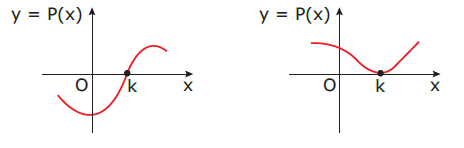
\includegraphics[scale=0.9]{Imagens/SLF1.png}
   
\end{figure}
\end{frame}

% Operações com Polinômios: Adição e Subtração
\begin{frame}{Operações com Polinômios: Adição e Subtração}
  \begin{block}{Regra Prática}<1->
    Nessas operações, basta adicionarmos ou subtrairmos os coeficientes dos \textbf{termos semelhantes}.
  \end{block}

  \pause

  \begin{exampleblock}{Exemplo da Apostila}<2->
    Considerar os polinômios:
    \[
      A(x) = 5x^4 - 3x^3 + 18x^2 - 9x + 12 \quad \text{e} \quad B(x) = x^4 + 23x^3 - 7x^2 + x + 3
    \]
    Calcule em sala:
    \begin{enumerate}
      \item $A(x) + B(x)$
      \item $A(x) - B(x)$
    \end{enumerate}
  \end{exampleblock}
\end{frame}

% Operações com Polinômios: Multiplicação
\begin{frame}{Operações com Polinômios: Multiplicação}
  \begin{block}{Regra Prática}<1->
    Multiplica-se cada termo de $A(x)$ por todos os termos de $B(x)$, reduzindo em seguida os termos semelhantes.
  \end{block}

  \pause

  \begin{alertblock}{Propriedade dos Graus}<2->
    \[
      \text{grau}(A \cdot B) = \text{grau}(A) + \text{grau}(B)
    \]
  \end{alertblock}

  \pause

  \begin{exampleblock}{Exemplo da Apostila}<3->
    Sejam $A(x) = x^2 - 3x + 2$ e $B(x) = 2x - 1$. Determine $A(x) \cdot B(x)$.
  \end{exampleblock}
\end{frame}

% Divisão pelo Método da Chave: Teorema
\begin{frame}{Divisão de Polinômios: Conceito}
  \begin{block}{Teorema da Divisão (Algoritmo de Euclides)}<1->
    Da divisão de dois polinômios $A(x)$ e $B(x)$ não nulos, obtêm-se os polinômios $Q(x)$ (quociente) e $R(x)$ (resto), tais que:
    \[
      A(x) = B(x) \cdot Q(x) + R(x)
    \]
  \end{block}

  \pause

  \begin{alertblock}{Condição para o Resto}<2->
    \[
      \text{grau}(R) < \text{grau}(B) \quad \text{ou} \quad R(x) = 0 \quad (\text{divisão exata})
    \]
  \end{alertblock}
\end{frame}

% Divisão pelo Método da Chave: Exemplo
\begin{frame}{Divisão pelo Método da Chave}
  \begin{exampleblock}{Exemplo Prático}
    Efetuar a divisão do polinômio $P(x) = 4x^3 + 2x^2 - x + 1$ pelo polinômio $B(x) = x^2 + 2x + 3$.
  \end{exampleblock}


\end{frame}

% Exercício Resolvido 01
\begin{frame}{Exercício Resolvido 01}
  \begin{exampleblock}{Exercício Resolvido 01 (UFMG)}
    O valor de $a$ para que $1 + \sqrt{2}$ seja raiz do polinômio $P(x) = x^3 + ax^2 + x + 1$ é:
    \vspace{0.3cm}
    \begin{columns}
      \column{0.5\linewidth}
      \begin{enumerate}[(A)]
        \item $-3$
        \item $-1$
      \end{enumerate}
      \column{0.5\linewidth}
      \begin{enumerate}[(A)]
        \setcounter{enumi}{2}
        \item $1$
        \item $3$
      \end{enumerate}
    \end{columns}
  \end{exampleblock}

  
\end{frame}

% Exercício Resolvido 02
\begin{frame}{Exercício Resolvido 02}
  \begin{exampleblock}{Exercício Resolvido 02 (UFES)}
    O polinômio $x^3 + ax^2 + bx + 7$, com coeficientes reais, é divisível por $x^2 + x + 1$. O valor da soma $a + b$ é igual a:
    \vspace{0.3cm}
    \begin{columns}
      \column{0.3\linewidth}
      \begin{enumerate}[(A)]
        \item $7$
        \item $14$
      \end{enumerate}
      \column{0.3\linewidth}
      \begin{enumerate}[(A)]
        \setcounter{enumi}{2}
        \item $15$
        \item $16$
      \end{enumerate}
      \column{0.3\linewidth}
      \begin{enumerate}[(A)]
        \setcounter{enumi}{4}
        \item $21$
      \end{enumerate}
    \end{columns}
  \end{exampleblock}

 
\end{frame}

\end{document}